
% Chapter Template
% Chapter Template
\setstretch{1}
\chapter{Conclusion}\thispagestyle{empty} % Main chapter title

\label{Chapter5} % Change X to a consecutive number; for referencing this chapter elsewhere, use \ref{ChapterX}

\lhead{Chapter 5. \emph{Conclusion}} % Change X to a consecutive number; this is for the header on each page - perhaps a shortened title
\setstretch{2}
%----------------------------------------------------------------------------------------
%	SECTION 1
%----------------------------------------------------------------------------------------

\section{Conclusion}
The work that has gone into the production and release of screenPerfect is not inconsiderable. As a creative project, code is a tricky thing to pin down. It must say something structurally, yet it reveals the internal architecture of its authors. Programming leaves loose ends. An excellent piece of software is likely to require input from a wide array of specialists in graphic design, interface development, and logic. There is an inevitable tendency to produce flaws - bugs - that cause the program to fail. Once complete, it is likely that finished software will fall out of fashion. Just as there is no way to call a piece of writing finished, because another word can always be added or cut loose, code is subject to scope creep. 

Code lives, like writing, in context and within an ecosystem. Code answers to its context. As Alexander Galloway says, without the machines that run it, code is without consequence \cite{galloway}. Within those machines, code may have a concrete effect on the world around it, and for that reason it continues to be valued. To code is to attempt to write a way of addressing the world, a single way that must take into consideration all the assumptions of people who tried to address the world before, and, with future-proofing, the world after. 

In Cixous' Laugh of the Medusa \parencite{cixous} she states that to be considered real, women must write for themselves. In my thesis, I have extended this to the world of code, and through it to computers: one must write after one's own interests, represent a possibility for what one believes can be real. I have done this by writing a tool that permits an array of interested parties to produce games without a reliance on what a game-engine maker thinks of as resources, and then extended it with hardware to support what I consider to be a straightforward installation path using materials from a not-for-profit, then sharing them publicly.

Writing a projection/presentation/game system has been work designed to address the problem of what, exactly, a game is, or what is a valuable piece of work. screenPerfect is designed to evaporate, leaving only the experience of its content to represent itself. The system does not judge content. It does not care where you serve your information, or to whom. The emphasis is on allowing an audience to experience things as quickly and easily as possible. Works produced using screenPerfect can be displayed anywhere a series of screens and a single server can be set up. This emphasis on experience moves the interaction sphere of art and gaming into the world. screenPerfect's impact is most felt at night, outdoors, or in temporary installations. The display of video-art and collaborative gameplay made possible through screenPerfect can be anywhere at all, and indeed works best at night, outdoors, in temporary installations. These are the new/old/new exhibits, the one-time-only parties, the experience that happens in a hard to access place but leaves no marks for future visitors to interpret.

The reflective portion of this research has been to address the question of what constitutes accessibility. At minimum, this is software which is straightforward for non-technical people to use. In addition, this includes attention paid to hardware to reduce the reliance on specialized technicians to exhibit and install interactive works, which otherwise are not terribly collectible \cite{lisanotes}. At the heart of screenPerfect is the idea that we can pull away from artificial distance and have instead on-site participation, unique experiences that project real, contemporary art into real, contemporary spaces.

At the outset, I asked a series of questions about capital, monetary and otherwise, creative practice, and preservation in the digital context. In the effort of designing screenPerfect, I have put forth a physical idea, which is that a small tool optimized to do one thing well is better than a tool that can do all things but requires a manual. I have suggested that a piece of software that addresses the needs of a specific group of curious people is likely to permit them to express themselves in a new medium, and I have issued the idea that a piece of hardware that boots when plugged in and serves that software in a reliable fashion might have a better half-life in a public context than one which needs to be custom installed to a diverse suite each time by hand. This is an effort to directly address the debate about games as art by circumvention: as we can see by visiting Cixous, any form of creative practice can be dismissed as wanking. The debate is in fact a longstanding form of access control. By giving people tools, we give them the ability to express themselves: if what they would like to say is then something personal, I believe there is value in that.

There are futher questions within my theory chapter, about the valuation of personal narratives as games, as economic or artistic practice. My conclusion to this is that it is not necessary to join the commercial order, but that if one does not display one's work, it is hard to say if the work has been done at all. This is the core of software. It hides until it breaks. A new direction could be to have software that obviously breaks, or that decays in an interesting fashion, and this leads to the glitch aesthetic, which is popular, and beautiful in its way. Another could be simply to understand that things which cannot be seen or quantified have nonetheless value, and to quantify that value on a different plane - efforts at this direction include Una Lee's Difference Engine poster, about what the participants of the first women-only game incubator achieved from participation in that incubator (Figure 5.1).

We live within a system of value and valuation, and I believe that it is unlikely we will overcome all elements of the system from within, an assertion supported by mathematicians like Gödel as much as feminists like Lorde. Systems cannot be internally resolved, but they can be regarded from outside, then circumvented. We can choose how much to engage with the system, and on what terms, and we can solve specific problems in the circumvention.

The effort proves the system incomplete, and in so doing, offers a wish for something better.

\clearpage
\begin{figure}[!ht]
\centering
  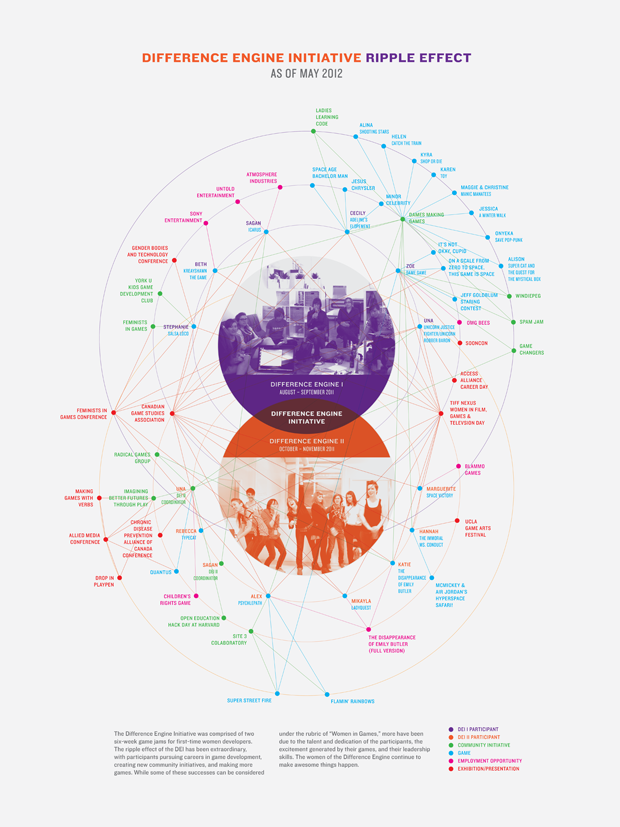
\includegraphics[width=0.8\textwidth]{DEIMayViz.png}
 \caption{Una Lee, Difference Engine Initiative Visualization, 2012}
\end{figure}
\clearpage